\chapter{Radioactivity and Nuclear Reactions}
\label{ch:radioactivity_reactions}

\begin{chapterintro}
\textbf{Chapter Objectives:} In this concluding chapter, we explore the physics and kinetics of spontaneous nuclear transformations and induced nuclear reactions. You will master the four natural disintegration modes ($\alpha, \beta^-, \beta^+, \gamma$); balance nuclear transmutations using the Soddy-Fajans conservation laws; solve the first-order differential decay equations for particle counts, mass, and activity; calculate half-lives and specific activities in Becquerels and Curies; and apply decay kinetics to archaeological radiocarbon dating and geological geochronology.
\end{chapterintro}

\section{Introduction to Radioactivity and Historical Foundations}

\begin{definitionbox}{Radioactivity}
\textbf{Radioactivity} is the spontaneous, exoenergetic physical process by which an unstable atomic nucleus (\textbf{parent nucleus}) undergoes an intrinsic restructuring or transmutation into a more stable nuclear configuration (\textbf{daughter nucleus}) accompanied by the emission of energetic nuclear particles ($\alpha$ or $\beta$) and/or high-energy electromagnetic radiation ($\gamma$).
\end{definitionbox}

\begin{historicalbox}{Becquerel, Marie Curie, and Soddy: Pioneers of Radioactivity}
\begin{minipage}{0.30\textwidth}
\centering
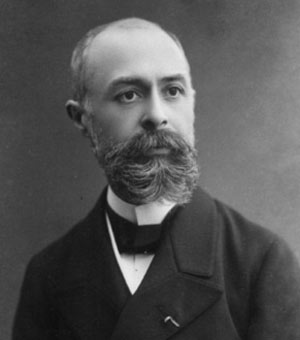
\includegraphics[width=0.92\textwidth]{images/becquerel.jpg}
\captionof{figure}{Henri Becquerel (1852--1908).}
\end{minipage}\hfill
\begin{minipage}{0.30\textwidth}
\centering
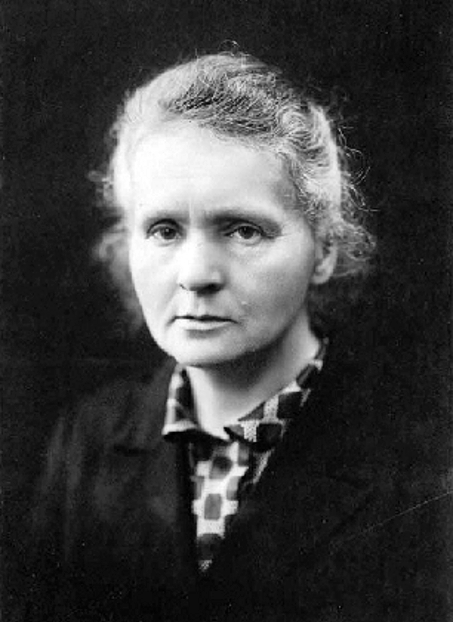
\includegraphics[width=0.92\textwidth]{images/curie.jpg}
\captionof{figure}{Marie Curie (1867--1934).}
\end{minipage}\hfill
\begin{minipage}{0.30\textwidth}
\centering
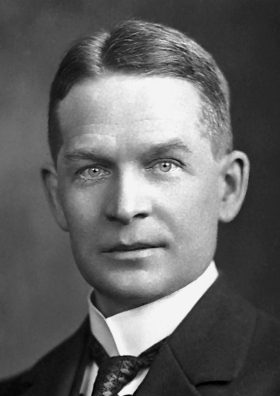
\includegraphics[width=0.92\textwidth]{images/soddy.jpg}
\captionof{figure}{Frederick Soddy (1877--1956).}
\end{minipage}

In 1896, French physicist Henri Becquerel accidentally discovered that uranium salts wrapped in opaque black paper spontaneously exposed photographic plates without sunlight. Marie Sk\l{}odowska-Curie coined the term \emph{radioactivity} and, alongside Pierre Curie, isolated the highly radioactive elements polonium and radium from pitchblende ore. In 1913, Frederick Soddy formulated the radioactive displacement laws, proving that radioactive decay transmutes one chemical element into another.
\end{historicalbox}

\section{Natural Radioactivity and Fundamental Decay Modes}

Unstable nuclei spontaneously decay via four primary physical mechanisms governed by nuclear instability (excess mass, excess neutrons, or excess protons):

\begin{figure}[htbp]
\centering
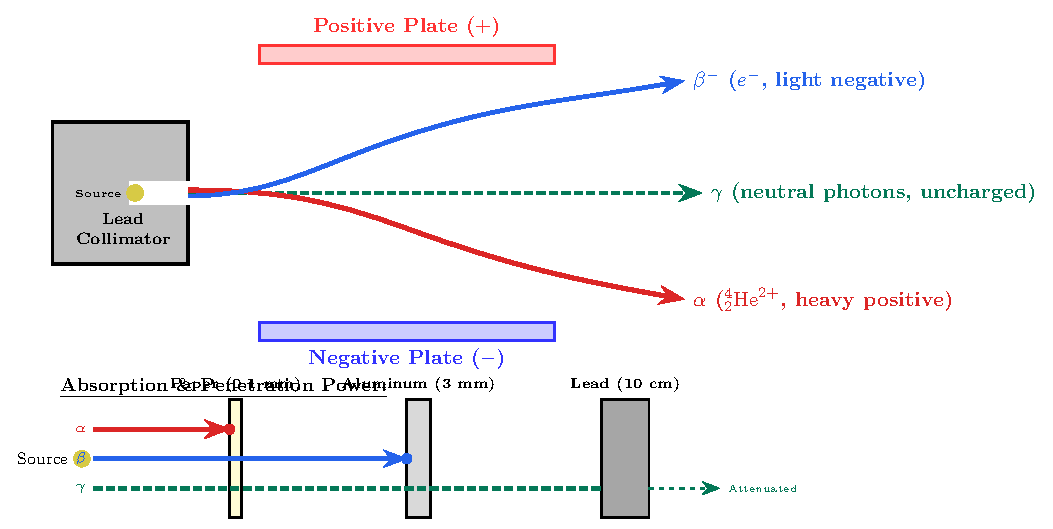
\includegraphics[width=0.88\textwidth]{figures/06_nuclear_deflection.pdf}
\caption{Top: Deflection of $\alpha$, $\beta^-$, and $\gamma$ rays in a transverse electric field. The heavy positive $\alpha$ particles bend gently toward the negative plate; light negative $\beta^-$ electrons bend sharply toward the positive plate; neutral $\gamma$ photons propagate undeflected. Bottom: Penetration power through paper ($0.1\ \mathrm{mm}$), aluminum ($3\ \mathrm{mm}$), and dense lead ($10\ \mathrm{cm}$).}
\label{fig:nuclear_deflection}
\end{figure}

\subsection{1. Alpha ($\alpha$) Disintegration}
Alpha decay occurs primarily in heavy radionuclides ($Z > 82, A > 200$) seeking to shed excess positive charge and mass. The parent nucleus expels a tightly bound Helium-4 nucleus ($\ce{^4_2He^{2+}}$):
\begin{equation}
\ce{^{A}_{Z}X -> ^{A-4}_{Z-2}Y + ^4_2He}.
\end{equation}
\begin{itemize}[leftmargin=1.5em,itemsep=2pt]
  \item \textbf{Displacement Law:} Mass number decreases by $4$ ($\Delta A = -4$); atomic number decreases by $2$ ($\Delta Z = -2$, shifting the element two columns to the left in the periodic table).
  \item \textbf{Canonical Example:} Alpha decay of Uranium-238 to Thorium-234:
  \[
  \ce{^{238}_{92}U -> ^{234}_{90}Th + ^4_2He}.
  \]
  \item \textbf{Physical Properties:} Alpha particles are massive ($m_\alpha \approx 4\ \mathrm{u}$) and carry charge $+2e$. They possess high linear energy transfer (LET) and intense ionizing power, but very low penetration: an ordinary sheet of paper ($0.1\ \mathrm{mm}$) or dead outer skin cells completely stops them.
\end{itemize}

\subsection{2. Beta-Minus ($\beta^-$) Disintegration}
Beta-minus decay occurs in **neutron-rich** nuclei located above the valley of nuclear stability ($N/Z$ ratio too high). Inside the nucleus, a neutron spontaneously converts into a proton via the weak nuclear interaction, emitting an energetic high-speed electron ($^0_{-1}e$) and an electron antineutrino ($\bar{\nu}_e$):
\begin{equation}
\ce{^1_0n -> ^1_1p + ^0_{-1}e + \bar{\nu}_e}.
\end{equation}
The nuclear transmutation equation is:
\begin{equation}
\ce{^{A}_{Z}X -> ^{A}_{Z+1}Y + ^0_{-1}e + \bar{\nu}_e}.
\end{equation}
\begin{itemize}[leftmargin=1.5em,itemsep=2pt]
  \item \textbf{Displacement Law:} Mass number remains invariant ($\Delta A = 0$); atomic number increases by $1$ ($\Delta Z = +1$, shifting the element one column to the right).
  \item \textbf{Canonical Example:} Beta decay of Carbon-14 into stable Nitrogen-14:
  \[
  \ce{^{14}_6C -> ^{14}_7N + ^0_{-1}e + \bar{\nu}_e}.
  \]
  \item \textbf{Physical Properties:} $\beta^-$ particles are electrons traveling at relativistic speeds ($v \sim 0.9\,c$). They penetrate several meters of air or several millimeters of biological tissue, but are halted by a thin aluminum plate ($3\text{--}5\ \mathrm{mm}$).
\end{itemize}

\subsection{3. Beta-Plus ($\beta^+$) Disintegration (Positron Emission)}
Beta-plus decay occurs in **proton-rich** nuclei located below the valley of stability ($N/Z$ ratio too low). A nuclear proton converts into a neutron, emitting a **positron** ($^0_{+1}e$, the antimatter counterpart of the electron) and an electron neutrino ($\nu_e$):
\begin{equation}
\ce{^1_1p -> ^1_0n + ^0_{+1}e + \nu_e}.
\end{equation}
The nuclear transmutation equation is:
\begin{equation}
\ce{^{A}_{Z}X -> ^{A}_{Z-1}Y + ^0_{+1}e + \nu_e}.
\end{equation}
\begin{itemize}[leftmargin=1.5em,itemsep=2pt]
  \item \textbf{Displacement Law:} Mass number remains invariant ($\Delta A = 0$); atomic number decreases by $1$ ($\Delta Z = -1$, shifting the element one column to the left).
  \item \textbf{Canonical Example:} Fluorine-18 decay utilized in Positron Emission Tomography (PET scans):
  \[
  \ce{^{18}_9F -> ^{18}_8O + ^0_{+1}e + \nu_e}.
  \]
  \item \textbf{Positron Annihilation:} Upon encountering an ambient orbital electron ($e^-$), the emitted positron undergoes immediate matter-antimatter annihilation, producing two diametrically opposed $511\ \mathrm{keV}$ gamma photons:
  \[
  \ce{^0_{+1}e + ^0_{-1}e -> 2\,\gamma} \quad (E_\gamma = m_e c^2 = 0.511\ \mathrm{MeV}).
  \]
\end{itemize}

\subsection{4. Gamma ($\gamma$) Electromagnetic De-excitation}
Following an $\alpha$ or $\beta$ transition, the daughter nucleus is frequently left in a quantum-mechanically excited metastable nuclear state, designated by an asterisk $[^{A}_{Z}\mathrm{Y}]^*$. The nucleus returns to its ground state by emitting one or more ultra-high-energy electromagnetic photons ($\gamma$-rays):
\begin{equation}
\ce{[^{A}_{Z}Y]^* -> ^{A}_{Z}Y + \gamma}.
\end{equation}
\begin{itemize}[leftmargin=1.5em,itemsep=2pt]
  \item \textbf{Displacement Law:} Neither mass number nor atomic number changes ($\Delta A = 0, \Delta Z = 0$). Gamma emission is a pure energetic de-excitation.
  \item \textbf{Physical Properties:} Gamma rays are uncharged electromagnetic photons of extremely short wavelength ($\lambda < 10^{-11}\ \mathrm{m}$) and high energy ($E_\gamma \sim 0.1\text{--}10\ \mathrm{MeV}$). They possess tremendous penetration power, requiring several centimeters of dense lead ($\mathrm{Pb}$) or several meters of reinforced concrete for radiation shielding.
\end{itemize}

\section{Conservation Laws in Nuclear Reactions (Soddy-Fajans Laws)}

Every nuclear transmutation, whether natural or artificially induced, obeys the strict **Soddy-Fajans conservation principles**:

\begin{lawbox}{The Soddy-Fajans Conservation Laws}
For any general nuclear reaction:
\begin{equation}
\ce{^{A_1}_{Z_1}X_1 + ^{A_2}_{Z_2}X_2 -> ^{A_3}_{Z_3}X_3 + ^{A_4}_{Z_4}X_4 + \dots}
\end{equation}
\begin{enumerate}[leftmargin=1.5em,itemsep=3pt]
  \item \textbf{Conservation of Nucleon Mass Number $A$:} The sum of mass numbers of the reactants equals the sum of mass numbers of the products:
  \begin{equation}
  \sum A_{\text{reactants}} = \sum A_{\text{products}} \iff A_1 + A_2 = A_3 + A_4 + \dots
  \end{equation}
  \item \textbf{Conservation of Electric Charge Number $Z$:} The algebraic sum of atomic numbers (nuclear charges) is strictly conserved:
  \begin{equation}
  \sum Z_{\text{reactants}} = \sum Z_{\text{products}} \iff Z_1 + Z_2 = Z_3 + Z_4 + \dots
  \end{equation}
  \item \textbf{Conservation of Total Relativistic Energy and Momentum:} Total energy (including rest mass energy $m c^2$) and total linear momentum are conserved.
\end{enumerate}
\end{lawbox}

\section{Artificial Nuclear Reactions and Transmutations}

Artificial nuclear reactions are induced by bombarding a stationary target nucleus with accelerated particles (protons, alpha particles, deuterons, or thermal neutrons).

\subsection{1. Compact Reaction Notation}
Nuclear reactions are frequently written in the condensed notation:
\begin{equation}
\text{Target Nuclide}\;(\text{Incident Projectile},\;\text{Ejected Particle})\;\text{Residual Nuclide}.
\end{equation}
\begin{itemize}[leftmargin=1.5em,itemsep=3pt]
  \item \textbf{Rutherford's Transmutation (1919):}
  \[
  \ce{^{14}_7N + ^4_2He -> ^{17}_8O + ^1_1p} \iff \ce{^{14}_7N}(\alpha, p)\ce{^{17}_8O}.
  \]
  \item \textbf{Chadwick's Neutron Discovery (1932):}
  \[
  \ce{^9_4Be + ^4_2He -> ^{12}_6C + ^1_0n} \iff \ce{^9_4Be}(\alpha, n)\ce{^{12}_6C}.
  \]
  \item \textbf{Joliot-Curie Artificial Radioactivity (1934):}
  \[
  \ce{^{27}_{13}Al + ^4_2He -> ^{30}_{15}P + ^1_0n} \iff \ce{^{27}_{13}Al}(\alpha, n)\ce{^{30}_{15}P}.
  \]
\end{itemize}

\subsection{2. Nuclear Fission}
Heavy fissile nuclides like Uranium-235 ($\ce{^{235}_{92}U}$) or Plutonium-239 ($\ce{^{239}_{94}Pu}$), when capturing a low-energy thermal neutron ($v \approx 2200\ \mathrm{m/s}$), form an unstable compound nucleus that violently ruptures into two lighter fission fragments and $2$ to $3$ fast secondary neutrons:
\begin{equation}
\ce{^{235}_{92}U + ^1_0n -> [^{236}_{92}U]^* -> ^{141}_{56}Ba + ^{92}_{36}Kr + 3\,^1_0n} + 200\ \mathrm{MeV}.
\end{equation}
Because the reaction produces more neutrons than it consumes ($k > 1$), it sustains an exponential **nuclear chain reaction**, harnessed constructively in nuclear power reactors or destructively in atomic weapons.

\subsection{3. Thermonuclear Fusion}
At extreme temperatures ($T \sim 10^8\ \mathrm{K}$), light nuclei overcome their repulsive Coulomb barrier to fuse into heavier, more tightly bound nuclei:
\begin{equation}
\ce{^2_1H + ^3_1H -> ^4_2He + ^1_0n} + 17.59\ \mathrm{MeV}.
\end{equation}
Thermonuclear fusion powers the Sun and main-sequence stars and represents the ultimate aspiration of clean commercial fusion energy research (ITER, tokamak reactors).

\section{Kinetics of Radioactive Decay}

Radioactive disintegration is a stochastic quantum process: it is impossible to predict when an individual nucleus will decay, but for a macroscopic sample containing $N(t)$ identical nuclei, the decay rate is strictly proportional to the number of parent nuclei present.

\subsection{1. The Law of Radioactive Decay}

\begin{lawbox}{First-Order Radioactive Decay Law}
The instantaneous disintegration rate of a radionuclide is governed by the first-order differential equation:
\begin{equation}
\frac{\dd N(t)}{\dd t} = -\lambda \cdot N(t),
\end{equation}
where $\lambda > 0$ is the **decay constant** (disintegration constant), representing the intrinsic probability of decay per nucleus per unit time ($[\lambda] = \mathrm{s^{-1}}, \mathrm{min^{-1}}, \mathrm{h^{-1}}, \mathrm{yr^{-1}}$).
\end{lawbox}

\paragraph{Mathematical Derivation.}
Separating variables:
\[
\frac{\dd N}{N} = -\lambda\,\dd t.
\]
Integrating both sides from $t = 0$ (where $N(0) = N_0$) to time $t$:
\[
\int_{N_0}^{N(t)} \frac{\dd N'}{N'} = -\lambda \int_0^t \dd t' \implies \ln\left( \frac{N(t)}{N_0} \right) = -\lambda t.
\]
Exponentiating both sides:
\begin{equation}
\mathbf{N(t) = N_0\,e^{-\lambda t}}.
\end{equation}

\begin{figure}[htbp]
\centering
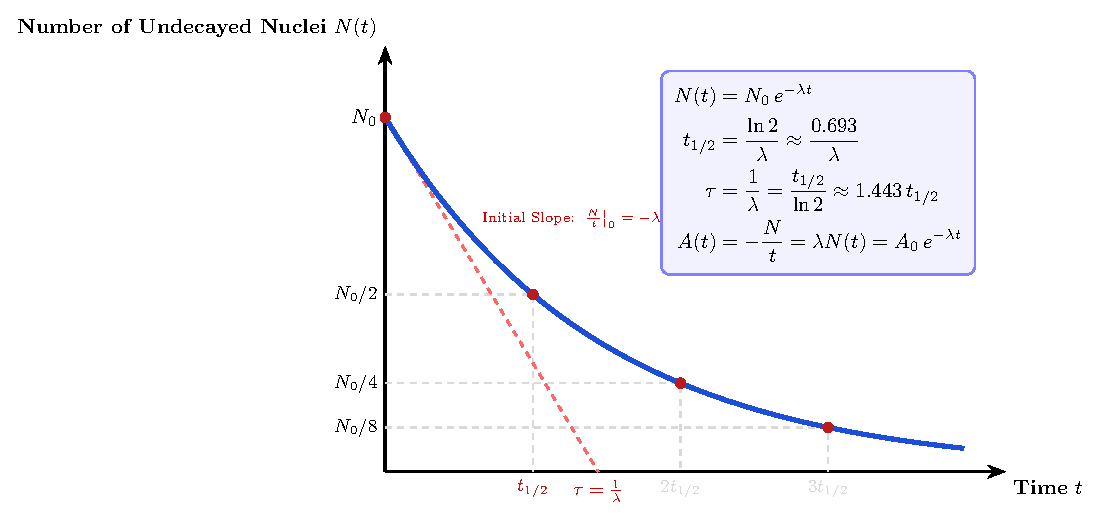
\includegraphics[width=0.88\textwidth]{figures/07_decay_kinetics.pdf}
\caption{Kinetics of radioactive decay. The population of undecayed nuclei decreases by half with every elapsed half-life $t_{1/2}$. The initial tangent line at $t=0$ intersects the time axis at the mean nuclear lifetime $\tau = 1/\lambda$.}
\label{fig:decay_kinetics}
\end{figure}

Because the mass $m(t)$ and amount of substance $n(t)$ of the radionuclide are directly proportional to particle count ($N = \frac{m}{M} N_A = n N_A$), the decay law applies identically to mass and moles:
\begin{equation}
m(t) = m_0\,e^{-\lambda t}, \qquad n(t) = n_0\,e^{-\lambda t}.
\end{equation}

\subsection{2. Radioactive Half-Life ($t_{1/2}$ or $T$)}

\begin{definitionbox}{Radioactive Half-Life}
The **radioactive half-life** $t_{1/2}$ (or \emph{period} $T$) is the time required for exactly one-half of the initial radioactive nuclei in a sample to disintegrate:
\begin{equation}
N(t_{1/2}) \eqdef \frac{N_0}{2}.
\end{equation}
\end{definitionbox}

Substituting into the decay law:
\[
\frac{N_0}{2} = N_0\,e^{-\lambda t_{1/2}} \implies e^{\lambda t_{1/2}} = 2 \implies \lambda \cdot t_{1/2} = \ln 2.
\]

\begin{lawbox}{Relationship Between Half-Life and Decay Constant}
\begin{equation}
\mathbf{t_{1/2} = \frac{\ln 2}{\lambda} \approx \frac{0.693\,147}{\lambda}}, \qquad \mathbf{\lambda = \frac{\ln 2}{t_{1/2}}}.
\end{equation}
After $k$ elapsed half-lives ($t = k \cdot t_{1/2}$), the remaining population is:
\begin{equation}
N(t) = N_0 \left(\frac{1}{2}\right)^k = \frac{N_0}{2^{t / t_{1/2}}}.
\end{equation}
\end{lawbox}

\subsection{3. Mean Nuclear Lifetime ($\tau$)}
The average lifetime of an individual radioactive nucleus before disintegration is:
\begin{equation}
\tau \eqdef \frac{1}{\lambda} = \frac{t_{1/2}}{\ln 2} \approx 1.4427 \cdot t_{1/2}.
\end{equation}
At time $t = \tau$, the population has dropped to $N(\tau) = N_0 / e \approx 0.3679\,N_0$ ($36.8\%$ remaining). Geometrically, $\tau$ is the intercept of the initial tangent line on the time axis (see Figure~\ref{fig:decay_kinetics}).

\section{Radioactive Activity ($A$) and Measurement Units}

\begin{definitionbox}{Radioactive Activity ($A$)}
The **radioactive activity** $A(t)$ of a sample is defined as the absolute rate of nuclear disintegrations occurring within the sample per unit time:
\begin{equation}
A(t) \eqdef -\frac{\dd N(t)}{\dd t} = \lambda \cdot N(t).
\end{equation}
At initial time $t = 0$: $A_0 = \lambda N_0$.
The activity decays following the identical exponential law:
\begin{equation}
\mathbf{A(t) = A_0\,e^{-\lambda t}}.
\end{equation}
\end{definitionbox}

\subsection{Units of Radioactivity}
\begin{itemize}[leftmargin=1.5em,itemsep=4pt]
  \item \textbf{The Becquerel ($\mathrm{Bq}$):} The official SI unit of radioactivity.
  \begin{equation}
  1\ \mathrm{Bq} \eqdef 1\ \text{disintegration per second}\ (\mathrm{dps}).
  \end{equation}
  \item \textbf{The Curie ($\mathrm{Ci}$):} Historical non-SI unit, originally defined as the activity of $1.00\ \mathrm{g}$ of pure Radium-226 ($\ce{^{226}_{88}Ra}$):
  \begin{equation}
  1\ \mathrm{Ci} \eqdef 3.7 \times 10^{10}\ \mathrm{Bq} = 3.7 \times 10^{10}\ \mathrm{dps} = 37\ \mathrm{GBq}.
  \end{equation}
  Decimal submultiples are universally used in medicine and industry:
  \begin{align*}
  1\ \mathrm{mCi} &= 10^{-3}\ \mathrm{Ci} = 3.7 \times 10^7\ \mathrm{Bq} = 37\ \mathrm{MBq}, \\
  1\ \mu\mathrm{Ci} &= 10^{-6}\ \mathrm{Ci} = 3.7 \times 10^4\ \mathrm{Bq} = 37\ \mathrm{kBq}.
  \end{align*}
\end{itemize}

\subsection{Specific Activity ($a_s$)}
The **specific activity** $a_s$ is the activity per unit mass of the pure radioactive isotope:
\begin{equation}
a_s \eqdef \frac{A}{m} = \frac{\lambda N}{m} = \frac{\lambda \left(\frac{m}{M} N_A\right)}{m} = \frac{\lambda N_A}{M} = \frac{\ln 2 \cdot N_A}{t_{1/2} \cdot M}, \qquad [a_s] = \mathrm{Bq\cdot g^{-1}} \quad (\text{or } \mathrm{Bq\cdot kg^{-1}}).
\end{equation}

\section{Applications of Radioactivity and Radiometric Dating}

\subsection{1. Archaeological Radiocarbon Dating ($^{14}\mathrm{C}$)}
Carbon-14 ($\ce{^{14}_6C}$) is continuously produced in the upper atmosphere by cosmic-ray neutrons bombarding Nitrogen-14:
\[
\ce{^{14}_7N + ^1_0n -> ^{14}_6C + ^1_1p}.
\]
The $^{14}\mathrm{C}$ rapidly oxidizes to $\ce{^{14}CO_2}$, entering the global biological carbon cycle through plant photosynthesis. In all living organisms, a dynamic metabolic equilibrium maintains a constant isotopic ratio:
\[
\left(\frac{\ce{^{14}C}}{\ce{^{12}C}}\right)_{\text{living}} \approx 1.2 \times 10^{-12} \iff A_0 \approx 15.3\ \text{disintegrations per minute per gram of carbon}\ (\mathrm{dpm\cdot g^{-1}}).
\]
When an organism dies, carbon assimilation abruptly ceases. The trapped $^{14}\mathrm{C}$ undergoes spontaneous $\beta^-$ decay ($t_{1/2} = 5730\ \mathrm{yr}$):
\[
\ce{^{14}_6C -> ^{14}_7N + ^0_{-1}e + \bar{\nu}_e}.
\]
Measuring the residual specific activity $A(t)$ of an archaeological specimen allows determination of its post-mortem age $t$:

\begin{lawbox}{Radiocarbon Age Equation}
\begin{equation}
t = \frac{1}{\lambda} \ln\left( \frac{A_0}{A(t)} \right) = \frac{t_{1/2}}{\ln 2} \ln\left( \frac{A_0}{A(t)} \right).
\end{equation}
\end{lawbox}

\subsection{2. Geological Rock Dating (Uranium-Lead Isochron)}
Uranium-238 ($\ce{^{238}U}$, $t_{1/2} = 4.468 \times 10^9\ \mathrm{yr}$) decays through a multi-step radioactive decay chain terminating at stable Lead-206 ($\ce{^{206}Pb}$):
\[
\ce{^{238}_{92}U -> ^{206}_{82}Pb + 8\,^4_2He + 6\,^0_{-1}e}.
\]
For a closed zircon crystal mineral that incorporated Uranium but zero initial Lead during magma crystallization:
\[
N(\ce{^{238}U}) = N_0\,e^{-\lambda t}, \qquad N(\ce{^{206}Pb}) = N_0 - N(\ce{^{238}U}) = N(\ce{^{238}U})(e^{\lambda t} - 1).
\]
The geological crystallization age of the rock is:
\begin{equation}
t = \frac{1}{\lambda} \ln\left( 1 + \frac{N(\ce{^{206}Pb})}{N(\ce{^{238}U})} \right).
\end{equation}

\section{Comprehensive Worked Examples}

\begin{workedexample}{Balancing Nuclear Transmutations and Decay Chains}
\begin{enumerate}[leftmargin=1.4em,itemsep=3pt]
  \item Identify the unknown particle or nuclide $\ce{X}$ in each of the following nuclear reactions:
  \begin{enumerate}[leftmargin=1.2em,itemsep=2pt]
    \item $\ce{^{226}_{88}Ra -> ^{222}_{86}Rn + X_1}$,
    \item $\ce{^{60}_{27}Co -> ^{60}_{28}Ni + X_2 + \bar{\nu}_e}$,
    \item $\ce{^{22}_{11}Na -> ^{22}_{10}Ne + X_3 + \nu_e}$,
    \item $\ce{^{235}_{92}U + ^1_0n -> ^{95}_{38}Sr + ^{139}_{54}Xe + X_4}$.
  \end{enumerate}
  \item The natural radioactive decay chain of Uranium-238 ($\ce{^{238}_{92}U}$) terminates at stable Lead-206 ($\ce{^{206}_{82}Pb}$) after a series of successive $\alpha$ and $\beta^-$ decays:
  \[
  \ce{^{238}_{92}U -> ^{206}_{82}Pb + x\,^4_2He + y\,^0_{-1}e}.
  \]
  Determine the exact integer number of alpha particles ($x$) and beta-minus particles ($y$) emitted throughout the entire chain.
\end{enumerate}

\paragraph{Solution.}
\textbf{1. Balancing Nuclear Reactions via Soddy-Fajans Laws:}\\
\begin{enumerate}[leftmargin=1.2em,itemsep=3pt]
  \item $\ce{^{226}_{88}Ra -> ^{222}_{86}Rn + X_1}$:
  Mass balance: $226 = 222 + A_1 \implies A_1 = 4$.
  Charge balance: $88 = 86 + Z_1 \implies Z_1 = 2$.
  $\mathbf{X_1 = \ce{^4_2He}}$ ($\alpha$ particle).
  \item $\ce{^{60}_{27}Co -> ^{60}_{28}Ni + X_2 + \bar{\nu}_e}$:
  Mass balance: $60 = 60 + A_2 \implies A_2 = 0$.
  Charge balance: $27 = 28 + Z_2 \implies Z_2 = -1$.
  $\mathbf{X_2 = \ce{^0_{-1}e}}$ ($\beta^-$ particle / electron).
  \item $\ce{^{22}_{11}Na -> ^{22}_{10}Ne + X_3 + \nu_e}$:
  Mass balance: $22 = 22 + A_3 \implies A_3 = 0$.
  Charge balance: $11 = 10 + Z_3 \implies Z_3 = +1$.
  $\mathbf{X_3 = \ce{^0_{+1}e}}$ ($\beta^+$ particle / positron).
  \item $\ce{^{235}_{92}U + ^1_0n -> ^{95}_{38}Sr + ^{139}_{54}Xe + X_4}$:
  Reactants: $\sum A = 235 + 1 = 236$; $\sum Z = 92 + 0 = 92$.
  Products (known): $\sum A = 95 + 139 = 234$; $\sum Z = 38 + 54 = 92$.
  Missing mass: $A_4 = 236 - 234 = 2$. Missing charge: $Z_4 = 92 - 92 = 0$.
  Because free neutrons have $A = 1, Z = 0$, the missing piece corresponds to two free neutrons:
  $\mathbf{X_4 = 2\,\ce{^1_0n}}$.
\end{enumerate}

\textbf{2. Uranium-238 Decay Chain Disintegration Count:}\\
Applying the conservation equations to $\ce{^{238}_{92}U -> ^{206}_{82}Pb + x\,^4_2He + y\,^0_{-1}e}$:
\begin{itemize}[leftmargin=1.5em,itemsep=2pt]
  \item Conservation of mass number $A$:
  \[
  238 = 206 + 4x + 0y \implies 4x = 238 - 206 = 32 \implies \mathbf{x = 8}.
  \]
  Exactly **$8$ alpha particles** are emitted!
  \item Conservation of charge number $Z$:
  \[
  92 = 82 + 2x - 1y.
  \]
  Substituting $x = 8$:
  \[
  92 = 82 + 2(8) - y = 82 + 16 - y = 98 - y \implies y = 98 - 92 \implies \mathbf{y = 6}.
  \]
  Exactly **$6$ beta-minus particles** are emitted!
\end{itemize}
The complete net decay chain is:
\[
\ce{^{238}_{92}U -> ^{206}_{82}Pb + 8\,^4_2He + 6\,^0_{-1}e + 6\,\bar{\nu}_e}.
\]
\end{workedexample}

\begin{workedexample}{Kinetics, Activity, and Attenuation of a Cobalt-60 Teletherapy Source}
Cobalt-60 ($\ce{^{60}_{27}Co}$) is a standard radionuclide used in industrial radiography and medical cancer radiation therapy. Its radioactive half-life is $t_{1/2} = 5.271\ \mathrm{years}$. A newly manufactured hospital radiotherapy head contains an initial Cobalt-60 activity $A_0 = 4000\ \mathrm{Ci}$.
\begin{enumerate}[leftmargin=1.4em,itemsep=3pt]
  \item Compute the radioactive decay constant $\lambda$ of Cobalt-60 in $\mathrm{s^{-1}}$ and in $\mathrm{yr^{-1}}$.
  \item Calculate the initial mass $m_0$ of pure Cobalt-60 in the source ($M = 59.9338\ \mathrm{g\cdot mol^{-1}}$).
  \item Determine the residual activity $A(t)$ (in $\mathrm{Ci}$ and in $\mathrm{TBq}$) after $3.00\ \mathrm{years}$ of clinical operation.
  \item Calculate the time $t$ required for the activity to decline to $1000\ \mathrm{Ci}$ (a factor of $4$ reduction).
\end{enumerate}

\paragraph{Solution.}
\textbf{1. Decay Constant $\lambda$:}\\
Using $1\ \mathrm{yr} = 365.25\ \mathrm{d} \times 86\,400\ \mathrm{s/d} = 3.15576 \times 10^7\ \mathrm{s}$:
\[
\lambda\ [\mathrm{yr^{-1}}] = \frac{\ln 2}{t_{1/2}} = \frac{0.693\,147}{5.271\ \mathrm{yr}} \approx \mathbf{0.13150\ \mathrm{yr^{-1}}}.
\]
In SI units:
\[
\lambda\ [\mathrm{s^{-1}}] = \frac{0.13150\ \mathrm{yr^{-1}}}{3.15576 \times 10^7\ \mathrm{s\cdot yr^{-1}}} \approx \mathbf{4.167 \times 10^{-9}\ \mathrm{s^{-1}}}.
\]

\textbf{2. Initial Mass of the Source:}\\
Convert the initial activity from Curies to Becquerels ($1\ \mathrm{Ci} = 3.7 \times 10^{10}\ \mathrm{Bq}$):
\[
A_0 = 4000\ \mathrm{Ci} \times 3.7 \times 10^{10}\ \mathrm{Bq\cdot Ci^{-1}} = 1.480 \times 10^{14}\ \mathrm{Bq} = 148.0\ \mathrm{TBq}.
\]
Since $A_0 = \lambda N_0$, the number of $\ce{^{60}Co}$ nuclei is:
\[
N_0 = \frac{A_0}{\lambda} = \frac{1.480 \times 10^{14}\ \mathrm{s^{-1}}}{4.167 \times 10^{-9}\ \mathrm{s^{-1}}} \approx 3.5517 \times 10^{22}\ \text{nuclei}.
\]
The initial mass of pure Cobalt-60 is:
\[
m_0 = \frac{N_0}{N_A} \times M = \frac{3.5517 \times 10^{22}}{6.02214 \times 10^{23}\ \mathrm{mol^{-1}}} \times 59.9338\ \mathrm{g\cdot mol^{-1}} \approx \mathbf{3.535\ \mathrm{g}}.
\]
A minuscule sample of only $3.54\ \mathrm{g}$ produces a colossal radiation activity of $4000\ \mathrm{Ci}$!

\textbf{3. Activity After $3.00\ \mathrm{Years}$:}\\
Applying the exponential decay law $A(t) = A_0\,e^{-\lambda t}$:
\[
A(3.00\ \mathrm{yr}) = 4000\ \mathrm{Ci} \times e^{-0.13150 \times 3.00} = 4000 \times e^{-0.3945} = 4000 \times 0.6740 \approx \mathbf{2696\ \mathrm{Ci}}.
\]
In Terabecquerels:
\[
A(3.00\ \mathrm{yr}) = 2696\ \mathrm{Ci} \times 3.7 \times 10^{10}\ \mathrm{Bq\cdot Ci^{-1}} \approx \mathbf{99.75\ \mathrm{TBq}}.
\]

\textbf{4. Time for Activity to Drop to $1000\ \mathrm{Ci}$:}\\
Notice that:
\[
\frac{A(t)}{A_0} = \frac{1000}{4000} = \frac{1}{4} = \left(\frac{1}{2}\right)^2.
\]
Because the activity drops by a factor of 4, exactly $k = 2$ half-lives have elapsed:
\[
t = 2 \times t_{1/2} = 2 \times 5.271\ \mathrm{yr} = \mathbf{10.542\ \mathrm{years}}.
\]
The source activity drops to $25\%$ in approximately $10.5$ years.
\end{workedexample}

\begin{workedexample}{Archaeological Radiocarbon Dating of an Ancient Artifact}
During an archaeological excavation of an ancient royal tomb, researchers discover a fragment of wooden furniture. A $1.00\ \mathrm{g}$ sample of purified elemental carbon extracted from the wood displays a measured beta activity of $4.18\ \text{disintegrations per minute}\ (\mathrm{dpm})$. Modern living tree wood displays a standard equilibrium carbon-14 activity of $A_0 = 15.30\ \mathrm{dpm\cdot g^{-1}}$. The half-life of Carbon-14 is $t_{1/2} = 5730\ \mathrm{years}$.
\begin{enumerate}[leftmargin=1.4em,itemsep=3pt]
  \item Determine the decay constant $\lambda$ of Carbon-14.
  \item Calculate the age of the wooden artifact and determine the historical era of the burial.
  \item What percentage of the initial Carbon-14 nuclei remains undecayed?
\end{enumerate}

\paragraph{Solution.}
\textbf{1. Decay Constant $\lambda$:}\\
\[
\lambda = \frac{\ln 2}{t_{1/2}} = \frac{0.693\,147}{5730\ \mathrm{yr}} \approx \mathbf{1.2097 \times 10^{-4}\ \mathrm{yr^{-1}}}.
\]

\textbf{2. Age of the Artifact:}\\
The measured specific activity is $A(t) = 4.18\ \mathrm{dpm\cdot g^{-1}}$, while the initial activity at the moment the tree was felled was $A_0 = 15.30\ \mathrm{dpm\cdot g^{-1}}$.
Applying the radiocarbon dating equation:
\[
A(t) = A_0\,e^{-\lambda t} \implies \frac{A(t)}{A_0} = e^{-\lambda t} \implies \ln\left( \frac{A(t)}{A_0} \right) = -\lambda t.
\]
Solving for the elapsed time $t$:
\[
t = \frac{1}{\lambda} \ln\left( \frac{A_0}{A(t)} \right) = \frac{1}{1.2097 \times 10^{-4}\ \mathrm{yr^{-1}}} \ln\left( \frac{15.30}{4.18} \right).
\]
Evaluating the natural logarithm:
\[
\frac{15.30}{4.18} \approx 3.6603 \implies \ln(3.6603) \approx 1.2975.
\]
The age of the wood is:
\[
t = \frac{1.2975}{1.2097 \times 10^{-4}} \approx \mathbf{10\,726\ \mathrm{years}}.
\]
The tree was harvested approximately $10\,700$ years ago (circa $8700\ \text{BCE}$), during the Neolithic period.

\textbf{3. Percentage of Undecayed $^{14}\mathrm{C}$ Remaining:}\\
The fraction remaining is:
\[
\frac{N(t)}{N_0} = \frac{A(t)}{A_0} = \frac{4.18}{15.30} \approx 0.2732 = \mathbf{27.32\%}.
\]
Approximately $72.68\%$ of the original Carbon-14 nuclei have disintegrated.
\end{workedexample}

\begin{workedexample}{Geological Geochronology: Uranium-Lead Mineral Dating}
A geologist analyzes a pristine zircon ($\mathrm{ZrSiO_4}$) crystal extracted from an ancient granite rock formation. High-precision thermal ionization mass spectrometry (TIMS) measures the present-day atom ratio of radiogenic Lead-206 to parent Uranium-238:
\[
\frac{N(\ce{^{206}Pb})}{N(\ce{^{238}U})} = 0.4280.
\]
Assuming the crystal contained no initial Lead at the time of magma solidification, and that no Uranium or Lead has leaked from the crystal lattice, calculate the geological crystallization age of the rock ($t_{1/2}(\ce{^{238}U}) = 4.468 \times 10^9\ \mathrm{years}$).

\paragraph{Solution.}
\textbf{1. Theoretical Geochronology Derivation:}\\
Each decayed $\ce{^{238}U}$ atom produces exactly one stable $\ce{^{206}Pb}$ atom:
\[
N_0 = N(\ce{^{238}U}) + N(\ce{^{206}Pb}).
\]
The remaining Uranium-238 population follows the decay law:
\[
N(\ce{^{238}U}) = N_0\,e^{-\lambda t}.
\]
Substituting $N_0$:
\[
N(\ce{^{238}U}) = \left[ N(\ce{^{238}U}) + N(\ce{^{206}Pb}) \right] e^{-\lambda t}.
\]
Dividing by $e^{-\lambda t}$ (multiplying by $e^{\lambda t}$):
\[
N(\ce{^{238}U})\,e^{\lambda t} = N(\ce{^{238}U}) + N(\ce{^{206}Pb}) \implies e^{\lambda t} = 1 + \frac{N(\ce{^{206}Pb})}{N(\ce{^{238}U})}.
\]
Taking the natural logarithm:
\[
\lambda t = \ln\left( 1 + \frac{N(\ce{^{206}Pb})}{N(\ce{^{238}U})} \right) \implies t = \frac{1}{\lambda} \ln\left( 1 + \frac{N(\ce{^{206}Pb})}{N(\ce{^{238}U})} \right).
\]

\textbf{2. Numerical Age Computation:}\\
The decay constant for Uranium-238 is:
\[
\lambda = \frac{\ln 2}{4.468 \times 10^9\ \mathrm{yr}} \approx 1.55135 \times 10^{-10}\ \mathrm{yr^{-1}}.
\]
The measured isotopic ratio is $0.4280$:
\[
1 + \frac{N(\ce{^{206}Pb})}{N(\ce{^{238}U})} = 1 + 0.4280 = 1.4280.
\]
Evaluating the natural logarithm:
\[
\ln(1.4280) \approx 0.356275.
\]
The age of the granite zircon crystal is:
\[
t = \frac{0.356275}{1.55135 \times 10^{-10}\ \mathrm{yr^{-1}}} \approx \mathbf{2.296 \times 10^9\ \mathrm{years}} = \mathbf{2.30\ \mathrm{billion\ years}}.
\]
The zircon crystal crystallized $2.30$ billion years ago during the Paleoproterozoic era of Earth's history.
\end{workedexample}
